\subsection{\textbf{RQ3:} How well do tools meet practitioner needs in resolving merge conflicts?}\label{RQ3}
Development tools need to be easy to use and provide contextualized pertinent information in a manner that is understandable.
To investigate how well current tools satisfy needs of practitioners when they resolve conflicts and which improvements would be most valuable to them, we asked our interview participants open-ended questions about how they resolve merge conflicts. 

Our results indicate that practitioners use a wide range of tools, with many directly using the Git command line interface. Our interview participants mentioned six different dimensions along which they would like improvements to tool support (see Table~\ref{survey_tool_needs}. 

We framed the survey questions to validate these improvement needs; participants ranked the above six needs.
We received 119 responses using a 5-point Likert scale to indicate the usefulness each type of tool improvement (1 being \textit{Not Useful}, 3 being \textit{Moderately Useful}, and 5 being \textit{Essential}).

In addition, we also asked participants which tools they use during conflict resolution.
We found 105 different tools from the 115 responses. Some mentioned generic responses such as \textit{``my text editor''}, which we create as a separate category.
%We group these generic responses together where semantically similar meanings exist. 
Table~\ref{survey_toolset} lists the top 10 most common tools used by participants to resolve merge conflicts.

In examining the list of these tools, we note that practitioners most often use basic tools (e.g. Git, Vim/vi, and Text Editor) to handle merge conflicts instead of employing specialized tools or plugins to modern IDEs. In this list, there is only one IDE (Eclipse (10 responses)), and three versioning specific toolsets (KDiff3 (9), Meld (8), SourceTree(8)). This indicates that practitioners are unable to leverage the functionalities provided by many research prototypes (e.g., Palantir~\cite{palantir}, Cyrstal~\cite{Brun2011}) that are specifically designed to facilitate proactive conflict detection, because they are built as plug-ins to modern IDEs. 

We next discuss the top four improvements from the survey responses. These are the responses that have a mean value higher than 3.0.

\begin{table}[!htbp]
\renewcommand{\arraystretch}{1.3}
\caption{Survey Participant Merge Toolsets (Top 10)}
\label{survey_toolset}
\centering
\begin{tabularx}{0.45\textwidth}{@{}r|Cl@{}}
\toprule
Tool & \# Participants & Description\\
\midrule
Git	& 37 & Version Control System\\
Vim/vi & 17 & Text Editor\\
Text Editor (unspecified) & 14 & Text Editor\\
Git Diff & 11 & Diffing Tool\\
GitHub & 11 & Website\\
Eclipse & 10 & IDE\\
KDiff3 & 9 & Diff \& Merge\\
Meld & 8 & Diff \& Merge\\
SourceTree & 8 & Git/Hg Desktop Client\\
Sublime Text & 7 & Text Editor\\
\bottomrule
\end{tabularx}
\end{table}

\Subsubsection{Better Usability}
%The right toolset is essential for efficiently developing solutions and resolving conflicts.
Usability is an important factor that determines whether a toolset supports or hinders the practitioner's workflows.
Our survey results indicate that better usability (I1) is the most desired improvement of the tool sets used for conflict resolution. 
%Based on the results of the survey, we found that practitioners rate usability as the most desired improvement for their current merge tools (I1).
While usability of a particular tool is important, the usability concerns become even more pertinent when they span across multiple tools that serve similar purpose and must operate in sync with each other.
Survey results indicate that participants use an average of 2.5 tools, and as many as 7 tools, to resolve merge conflicts.
%With multiple tools being used during merging and conflict resolution, toolset fragmentation is a real concern for practitioners.
For instance, in our interview P1 demonstrated how he typically resolved a merge conflict by using four different tools and said: 
\begin{displayquote}
\textit{``I have to jump around between tools and copy and paste version numbers from one to... See, this is why [toolset] integration matters.''}
\end{displayquote}

Switching across multiple tools while resolving a conflict is disruptive and comes at a cost. Psychology studies~\cite{Meiran2000}\cite{gopher2000switching} have shown that task switching reduces performance and causes mental fatigue. 
Gerald Weinberg highlighted that context switching arising from toolset fragmentation is a big problem in engineering teams~\cite{Weinberg1992}. 

%This frustration is understandable for practitioners whose workflows frequently get interrupted by tool switches. Psychology studies~\cite{Meiran2000}\cite{gopher2000switching} have found that task switching comes with costs in performance and mental fatigue, and, in 1992, Gerald Weinberg highlighted the problem of toolset fragmentation within engineering teams~\cite{Weinberg1992}. 

\Subsubsection{Better Exploration of Project History}
Developers have been known to use the historical data to understand code evolution and development process~\cite{mihai_lenses}.
However, while these systems (version control and bug trackers) contain a huge amount of meta-information about the evolution of the code and development process, it is not easy to find the right information. Currently, there is insufficient support for performing detailed analysis of how a code piece evolved over time. Better ways of exploring the project history (I3) was one of the top requested improvements in our survey. As P1 mentioned in the interview:
\begin{displayquote}
\textit{``Give me a way to explore the history. To drill down, to go back up, you know? To resurface and understand what happened.''}
\end{displayquote}


Currently, when performing any useful analysis it is easier to write stand alone scripts to extract the information that is needed to resolve conflicts. During the interview, P1 mentioned that he has written several scripts to locate particular historical commits that relate to a current merge conflict. Similarly, P9 described a tool, \texttt{git-diff}, that was developed by their team to add additional difference analysis functionality across branches:
\begin{displayquote}
\textit{``git-diff will just do the diff based on the SHAs... we're adding metadata and cherry picking, so the SHAs are always going to be changing... It also hooks into GitHub labels and uses the labels on the project to do some more advanced heuristics.''}
\end{displayquote}

While writing these scripts allow extraction of relevant data contextualized to the need, it also leads to a proliferation of multiple scripts that are written by individual developers and need to be maintained or integrated. This further adds to the problem where practitioners have to switch across multiple tools (and also run multiple scripts).

We are not the first in recognizing the in the support provided for analyzing development history among practitioners (~\cite{sun2015informationhistory, guo2016cold-start, yan2014miningcontracts}). However, it appears that practical applications current history exploration tools are still beyond the reach of practitioners. One of the reasons for this might be the simple set of text editors (and tool sets) that our study participants seem to prefer.

\todo{Need a story/ writeup/ quote for this}
\Subsubsection{Better Filtering of Less-Relevant Information}
%Version control systems (VCS) and bug tracking systems provide insufficient support for detailed analysis of software evolution and information retrieval~\cite{fischer2003release_history}.
%For software practitioners using \texttt{git} and other VCS, it is often easier to write scripts that accommodate their particular information needs by augmenting the capabilities of the VCS.
%During the interviews, P1 described writing several scripts in order to locate particular historical commits that relate to a current merge conflict.
%P9 also described a tool, \texttt{git-diff}, developed as part of their efforts to add additional difference analysis functionality across branches:
%\begin{displayquote}
%\textit{``git-diff will just do the diff based on the SHAs... we're adding metadata and cherry picking, so the SHAs are always going to be changing... It also hooks into GitHub labels and uses the labels on the project to do some more advanced heuristics.''}
%\end{displayquote}
%\todo{Shane: This transition is a bit rough}
%In our survey results, we see that practitioners rank \textit{better ways of filtering out less relevant information} (I2) as the second highest improvement needed in modern merge toolsets.
%This suggests that further work is needed to bring these capabilities from single-purpose scripts into common toolsets used by all practitioners.
%
%\Subsubsection{Better Exploration of Project History}
%Codoban et al.~\cite{mihai_lenses} introduced the concept of the \textit{Archeology Lens} to describe examining old development history to retrieve lost knowledge and postulated that additional tool support was needed in this context.
%We also find that practitioners consider history exploration to be a major area of improvement for development toolsets.
%Among survey participants, \textit{better ways of exploring project history} (I3) ranked as the third most important improvement needed.
%During our interviews, P1 said: 
%
%\begin{displayquote}
%\textit{``Give me a way to explore the history. To drill down, to go back up, you know? To resurface and understand what happened.''}
%\end{displayquote}
%
%The gap in support for analyzing development history among practitioner toolsets has previously been recognized by researchers~\cite{sun2015informationhistory, guo2016cold-start, yan2014miningcontracts}, however practical application of these efforts appear to have not yet reached practitioners.

\Subsubsection{Better Graphical Presentation of Information}
The usefulness of information is helped or hindered by the way in which it is presented to users.
In our survey results, we found that \textit{better graphical presentation of information} (I4) was ranked the fourth highest improvement needed in practitioner toolsets (mean: 3.14).
One of the survey participants' comment highlights this need for further toolset improvements:
\begin{displayquote}
\textit{``Tools don't make it easy to work with two arbitrary revisions side by side.''}
\end{displayquote}

In our interviews, several practitioners reported experiencing issues with inconsistent terminology, inconsistent visual metaphors (colors, notifications, etc.), and the organizational layout of different development tools.
The cost of context switching in software development is well-known to researchers~\cite{czerwinski2004taskswitching, li2007cost_of_context_switch, blackwell2002attentioninvestment, convertino2003dualview}, but the individual experiences of practitioners attempting to resolve merge conflicts isn't as well understood.
Practitioners conveyed that they would like to see tools that share a common language in both terminology and presentation, though survey participants indicated only a minor need for improvement in consistency of terminology. 

\begin{figure*}[!htbp]
\centering
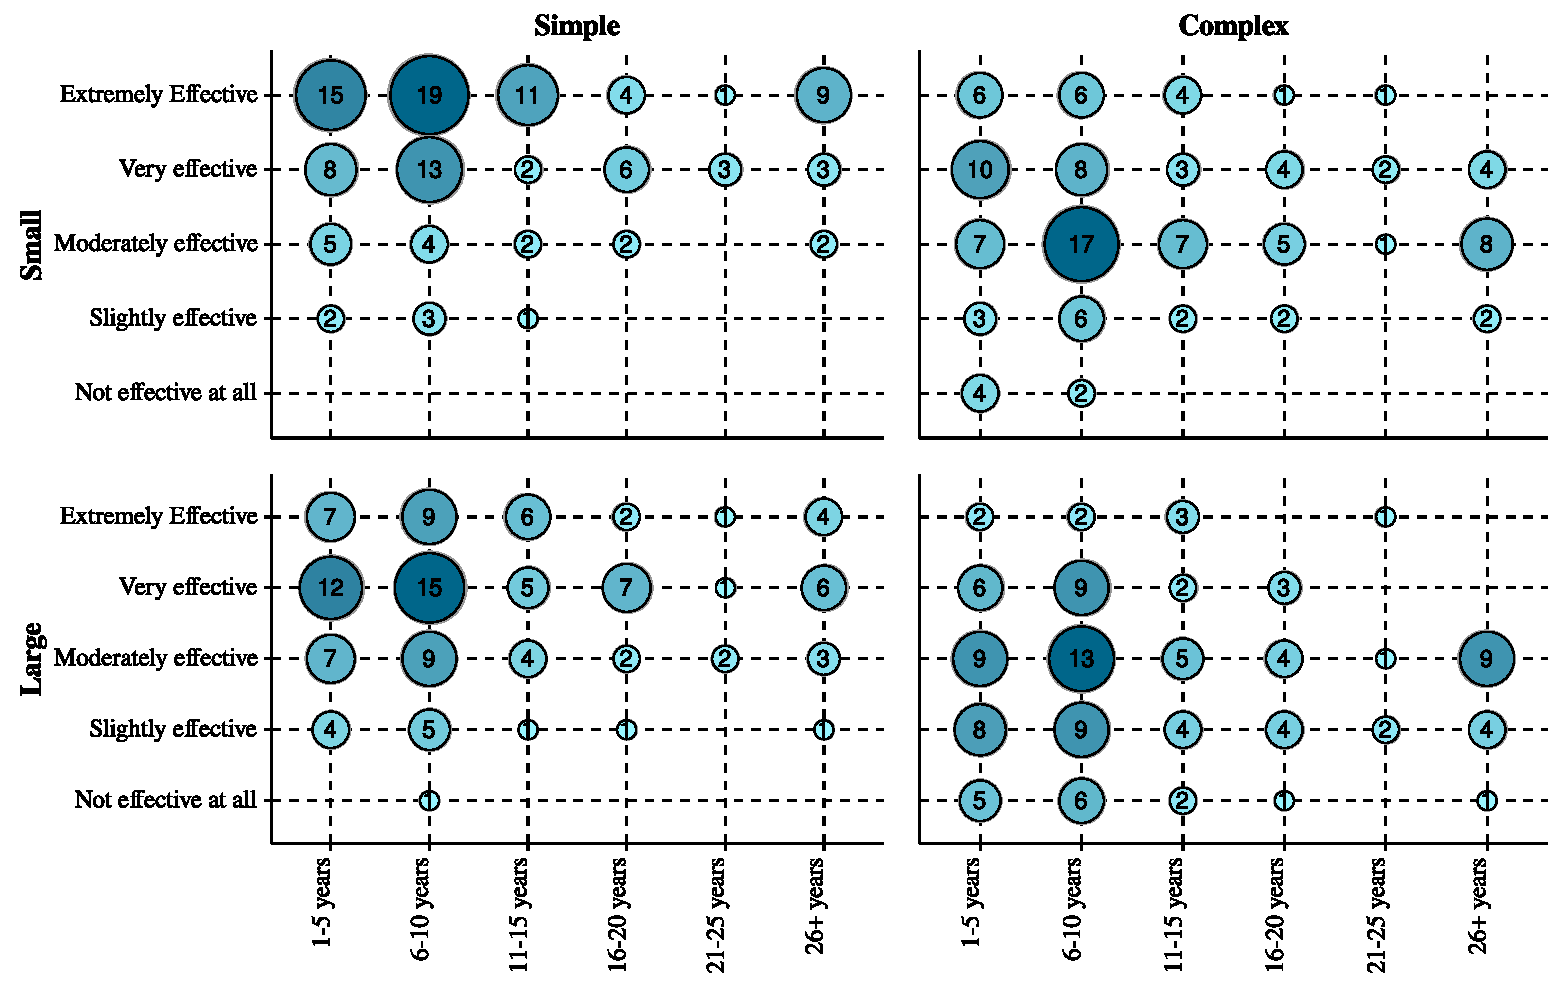
\includegraphics[width=\textwidth]{ConflictComplexityVsSize.pdf}
\caption{Effectiveness of practitioners' toolsets in supporting perceived size and complexity of merge conflicts, split on development experience. Bubble values indicate number of survey responses for effectiveness of a particular merge conflict size and complexity, and bubble size indicates the number of responses for comparison purposes.}
\label{size_vs_complexity}
\end{figure*}

\begin{table}[!htbp]
\renewcommand{\arraystretch}{1.3}
\caption{Practitioners' Trust in their Merging, History Exploration, and Conflict Resolution Tools\textsuperscript{i}}
\label{survey_tool_trust}
\centering
\begin{tabularx}{0.45\textwidth}{@{}r|*{10}{C}c@{}}
\toprule
Trust Level & Response Count & Response \%\\
\midrule
Completely & 20 & 16.52\\
A lot & 50 & 41.32\\
A moderate amount & 41 & 33.88\\
A little & 10 & 8.26\\
Not at all & 0 & 0.00\\
\bottomrule
	\multicolumn{3}{c}{\noindent\parbox[t]{7.8cm}{\vspace{-3px}\textsuperscript{i}\hspace{0.2em}Survey respondents answered on a 5-point Likert scale to indicate trust in their toolset (1 being \textit{Not at all} and 5 being \textit{Completely}).}}
\end{tabularx}
\end{table}

\Subsubsection{Tool Mistrust/Transparency}
Most merge tools attempt to resolve conflicts using a variety of algorithms, but revert to manual resolution when these algorithms fail.
Several interview participants indicated that they mistrust merge tools when they obscure the steps and rationale for particular results when resolving merge conflicts.
The opaque nature of history exploration tools was also found to be a source of practitioners' overall mistrust of their toolsets.
P4 commented that:
\begin{displayquote}
\textit{``I've never trusted the merge tools, in a way. Or the diff tools. It would always just make me skittish. So my overall perception is that I'm scared of them. Sometimes I'll even manually go and do the merge myself rather than use a tool. Just because I've had several times where it's a bad merge, and I broke some code.''}
\end{displayquote}

Based upon this theme of mistrust, we asked survey participants to rate the degree to which they trust their merging, history exploration, and conflict resolution tools.
We received 121 responses to this question, with a mean score of 3.66 placing the most common responses between \textit{a moderate amount} and \textit{a lot} of trust (Table~\ref{survey_tool_trust}).
Assuming that responses of \textit{a moderate amount}, \textit{a little}, or \textit{not at all} indicate some degree of mistrust, we find that 42.15\% of practitioners experience some gap in toolset trust.

However, the severity of toolset mistrust is not as significant as the interview results had lead us to assume.
Only 8.26\% of practitioners indicated that they trust their toolset \textit{a little} or \textit{not at all} (10 out of 121 responses).
The results of the survey are counterintuitive to our interview results, but appears to indicate that practitioners abandon mistrusted tools before all trust is lost in them.

\Subsubsection{Perceptions of Developer Tool Effectiveness}
The perceived size and complexity of merge conflicts affect the way in which practitioners plan, allocate, and enact resolutions.
To understand the degree to which these two factors impact practitioners' perceptions about the effectiveness of their toolsets, we asked survey participants to rate their toolset across four different merge conflict archetypes: (1) \textit{simple, small merge conflicts}, (2) \textit{simple, large merge conflicts}, (3) \textit{complex, small merge conflicts}, and (4) \textit{complex, large merge conflicts}.

Since individual participants have different toolsets, and consider different factors when determining the perceived size and complexity of a merge conflict, we instructed participants to rate their own toolset against these archetypes using their notion of what constitutes a simple vs. complex and small vs. large merge conflict.

Fig.~\ref{size_vs_complexity} provides a visual illustration of the results of this survey question.
Individual plots map participants' software development experience (horizontal axis) with their effectiveness responses for their merge toolsets (vertical axis) given the particular combination of size and complexity of merge conflicts (horizontal moves from \textit{simple} to \textit{complex}, and vertical moves from \textit{small} to \textit{large}).
The size and number contained within each bubble represent the total number of responses for that particular combination of factors.
For example, a practitioner with 6-10 years of experience that indicates that her merge toolset is \textit{Extremely Effective} for \textit{small, simple merge conflicts} would be represented in the largest bubble (containing 19) in the top-left plot.
That same practitioner would be represented in the largest bubble (containing 13) in the bottom-right plot if she indicated that her merge toolset was \textit{Moderately effective} for \textit{large, complex merge conflicts}.

Observing the overall trends when moving between plots, we find that practitioners perceive complexity to have a greater impact on the effectiveness of their merge toolsets than the size of merge conflicts.
The resulting trends are the same across all six groups of software development experience; decreasing effectiveness when moving from small to large, and even stronger decreases in effectiveness moving from simple to complex.
These results suggest that merge tools are currently better equipped to handle increases in the size of merge conflicts, but not as well equipped for increasing in complexity.
The increasing amount of code being developed in distributed environments means that scaling support in both dimensions is necessary to accommodate practitioners' needs.